\chapter{Results and Discussion}
\section{Baseline performance of ammonia concentration and colour level forecasting models}

\begin{figure}[h]
    \centering
    \begin{subfigure}{0.45\textwidth}
      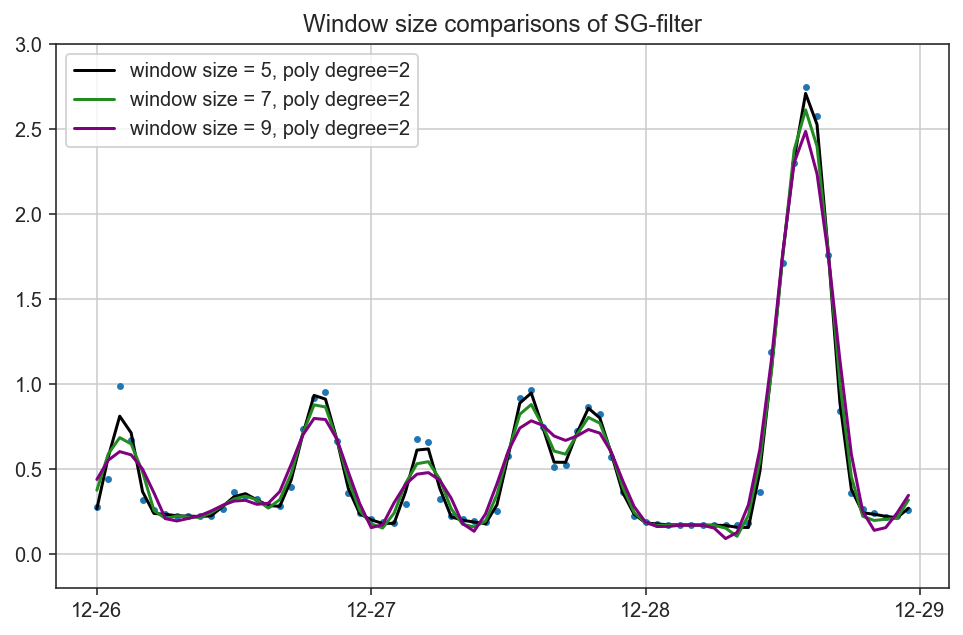
\includegraphics[width=\linewidth]{imgs/pre-processing/sg-filter.png}
      \caption{} \label{fig:smoothed-sg}
    \end{subfigure}%
    \hspace{2em}%   % maximize separation between the subfigures
    \begin{subfigure}{0.45\textwidth}
      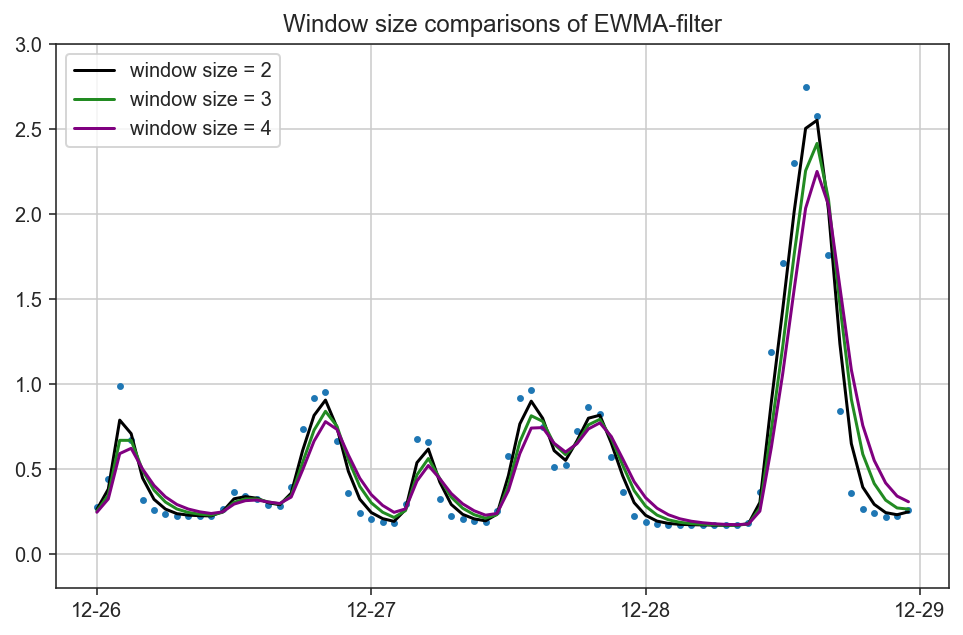
\includegraphics[width=\linewidth]{imgs/pre-processing/ew-filter.png}
      \caption{} \label{fig:smoothed-ew}
    \end{subfigure}%  
  \caption{Illustration of the influence of different polynomial degrees in the fitting of SG filter and the weigth decay with varied alpha values in EWMA filter.} \label{fig:smoothed}
  
\end{figure}
\subsection{Machine learning vs deep learning}
RF is used in this work as a representative tree-based modeling strategy because RF models have some major advantages over alternative tree-based models; notably, they require fewer hyperparameters for tuning, their performance is robust to hyperparameter changes, and they are less likely to suffer from overfitting (Breiman, 2001;Breiman, 2002 ;Chen and Guestrin, 2016;Fawagreh et al., 2014 ;Ke et al., 2017).
\section{Improved performance on forecasting models using data pre-processing techniques}
\section{Data enrichment via feature engineering based on effluent quality pattern}
\section{Design of model architecture through analyzing wastewater composition in sewer system}
